\chapter{Introduction}

The LDS church, it seems, is not exempt from the ever-increasing amount of data available to it. The Corpus of LDS General Conference talks (\emph{CLDSGCT}) increases in size bi-annually \citep{davies:gc}. Currently, it consists of over 1400 talks. This is a problem for members of the Church of Jesus Christ of Latter-day Saints because, even at a young age, they are admonished to study from these General Conference talks \citep{childrens_songbook}. The ability to navigate through the talks and make connections becomes increasingly difficult over time as the amount of information increases. Search systems are currently used to alleviate this burden. Recommendation systems may also serve to alleviate the information overload. The two methods may me implemented together as each take a differing approach to sifting through the data: search systems allow users to use search terms they know to find related documents, while recommender systems fulfill the role of recommending similar documents once one is located. This can be done on the web or in computer applications\footnote{LDS View (available at \url{http://ldsview.wordcruncher.com/}) is one such application.}.

At least 2 websites exist that allow members of the LDS community and the general public to search for talks by keyword, date of authorship, and speaker. They are (1) \url{LDS.org} which is the official website for the LDS church and (2) \url{scriptures.byu.edu} which is provided by Brigham Young University, a private school owned by the LDS church. \url{LDS.org} attempts to support topic-based searches (e.g. ``Talks on Faith''), but rather than searching by topic, users perform the search in a restricted ``talks'' space. The only way the site seems to allow users to search by topic is by year, so in order to find a list of all talks with a given topic tag (e.g. `Faith'), a user would need to load over 88 webpages. Both \url{LDS.org} and \url{scriptures.byu.edu} provide Lucene-like search functionality \citep{McCandless:2010:LAS:1893016,lucene:luke} and cross-references, but neither website provides a recommendation system nor a topical index for General Conference talks.

One way to find relevant documents is to use discovery-based techniques. These contrast with search-based techniques such as query search since results can be computed before a user actively makes a request. Readily available examples of are the use of product recommendation systems in commerce websites, for example \url{Amazon.com}. Specialized machine learning algorithms can automatically cluster data. Distance metrics measure how close each point within the cluster is to the others. From these distances, another algorithm can conclude which documents are most relevant for every other document. Depending on the application, clustering and ranking algorithms run online or offline. Recommendation systems are a form of discovery-based techniques. None appear to exist for \emph{CLDSGCT}.

This thesis will provide a recommendation system, \emph{RelRec}, for General Conference talks. The system will leverage inferred topical content when computing distances between documents. A side benefit of the system is that intermediate output could be used to provide a topical index in any website that has General Conference talks. The parameters of the the topic model will be inferred via \emph{(Collapsed) Gibbs Sampling} \citep{Porteous:2008:FCG:1401890.1401960}, although \emph{Variation Inference} could be used as well \citep{blei2006variational}. \emph{RelRec} will be an LDA + k-NN system, trained for General Conference talks. Since no recommendation system exists in this domain, it represents a novel application. In order to maintain a streamlined experience for website end-users, I will use offline forms of clustering and ranking. I will compare the performance of this system with that of an off-the-shelf \emph{TF-IDF} recommendation system, which represents a recognized baseline.

Since \emph{TF-IDF} makes no effort to differentiate between word senses and homographs, I hypothesize that \emph{RelRec} will outperform \emph{TF-IDF} in all benchmarks since token-topic assignments assigned by Collapsed Gibbs Sampling can be seen as a type of disambiguation.

The performance of \emph{RelRec} versus the \emph{TF-IDF} system will be measured across 3 metrics, 1 of which is a benchmark while the other two are comparative. The metrics will measure similarity, serendipity, and coverage. Based on the 1 benchmark, coverage, I will conclude which system is best. The similarity metric is meant to lend credence to either method, assuming that (1) the other is a well-accepted recommendation method and (2) the similarity level is high. I am open to modifying this portion of the thesis, of course; if I encounter other sensible metrics, I will consider applying them to the output of the two systems.




[You have probably heard that the amount of digital data is increasing at alarming rates each year. It is difficult to pin down the actual rate. BBC says ``Some say that about 90\% of all the data in the world today has been created in the past few years...According to computer giant IBM, 2.5 exabytes - that's 2.5 billion gigabytes (GB) - of data was generated every day in 2012. That's big by anyone's standards. ‘About 75\% of data is unstructured, coming from sources such as text, voice and video,’ says Mr Miles.'' I worked for a while at a company that stores backups of data. The amount of data they were storing reached 20 PB!]

With so much digital data, much of which is unstructured, it becomes necessary to assist users of data to sift through and learn from data leveraging computers to perform some of the tasks. One way to expose data is to allow users to search via query. Another way is by recommendation. In this thesis, I compare two recommendation systems and systematically select the best for use on the (unstructured) textual data I have, in preparation for potential enhancements to the website \url{http://scriptures.byu.edu} (hereafter, \emph{LDS Scripture Citation Index}, or simply \emph{LDS SCI}).




Before proceeding, I will preface that I endeavor to provide URL hyperlinks whenever possible so the reader can easily replicate this work, which seems fitting since this work aims to enhance the web community.

\section{About LDS Scripture Citation Index (SCI)}
\emph{LDS SCI} is available both on the web and on mobile devices. All forms have a search feature which utilizes a Lucene \citep{lucene:luke} back-end search which employs a \emph{TF-IDF} algorithm for ranking search matches for any query. Since the data made accessible by \emph{LDS SCI} is indexed and cataloged, it has some metadata which can be used as criteria in the filter, such as year, speaker or venue (e.g. General Conference).

\begin{figure}[hhhhhtb]
	\centering
		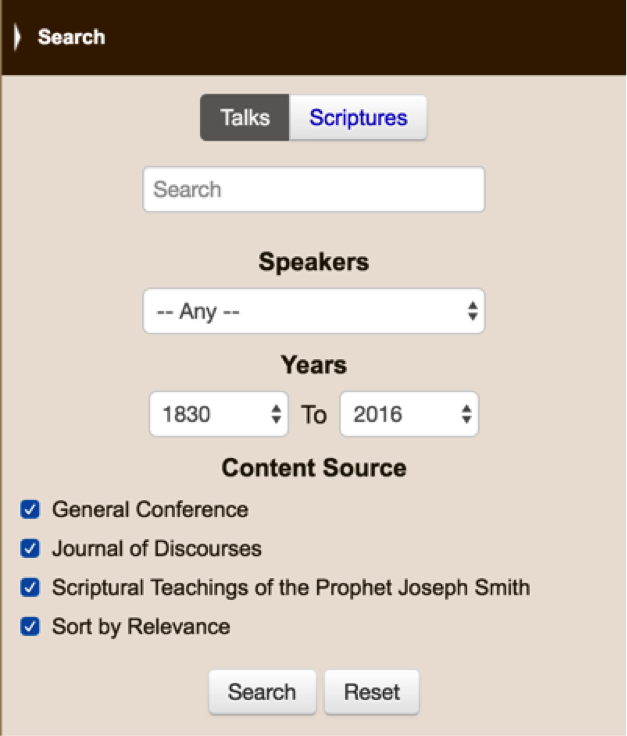
\includegraphics[width=3.5in,natwidth=310,natheight=442]{figures/sci_search.png}
		\caption[SCI \emph{TF-IDF} Search Results]{
			Samples results of a search provided to SCI Lucene search engine.
		}
	\label{fig:sci_search}
\end{figure}

Providing search capabilities is just one way \emph{LDS SCI} exposes their index. The area where \emph{LDS SCI} really shines is by its use of indexing. While an LDS discourse often has references placed in-line or at the end of the text, the reverse is not the case; LDS scriptures, including the ones found online at \url{https://www.lds.org/scriptures/}, have only footnotes. \emph{LDS SCI} has copies of LDS discourses and scriptures, indexes the references, then exposes that index in a searchable way. This allows users to reach discourses from scriptures (\url{LDS.org} does the reverse). While \url{LDS.org} provides discourse-based study or scripture-only study, \emph{LDS SCI} allows for an enhanced scripture-based study, starting at chapters of scripture leading to LDS discourses for potential clarification.

\emph{LDS SCI} is similar to \url{LDS.org} in that users can use them to read both scriptures and discourses. However, \emph{LDS SCI} exposes discourses pre-dating 1971, including those published in the Journal of Discourses in the 1800’s while \url{LDS.org} focuses on those published after 1971. [Related to \emph{LDS SCI} is a geographical version of scriptures \url{http://scriptures.byu.edu/mapscrip/} where users can read scriptures (Biblical and non-biblical) and see a Google Earth view of the related area(s).]

\section{Motivation}
While the \emph{LDS SCI} is helpful for the aspiring erudite (of LDS content), there is currently no recommendation system for the discourses: when a user finds an interesting discourse, there is no simple way to find similar/related discourse. Although the LDS website has some modern General Conference (GC) discourses tagged with topics, such topics are currently provided on a per-year basis only, so the discourses tagged with each topic tend to be sparse. This works when members of the LDS church want to focus on the most recent discourses only. Even with URL manipulation, an attempt to expose topics for all GC discourses rather than by year does not work (\url{https://www.lds.org/general-conference/topics/2015/10} vs. \url{https://www.lds.org/general-conference/topics/})--it results in the topic index for the most recent session of GC. Sparseness for the discourses in a given topic are apparent in the image--most topics only have 1 associated discourse and therefore have no number next to the topic’s title:

\begin{figure}[hhhhhtb]
	\centering
		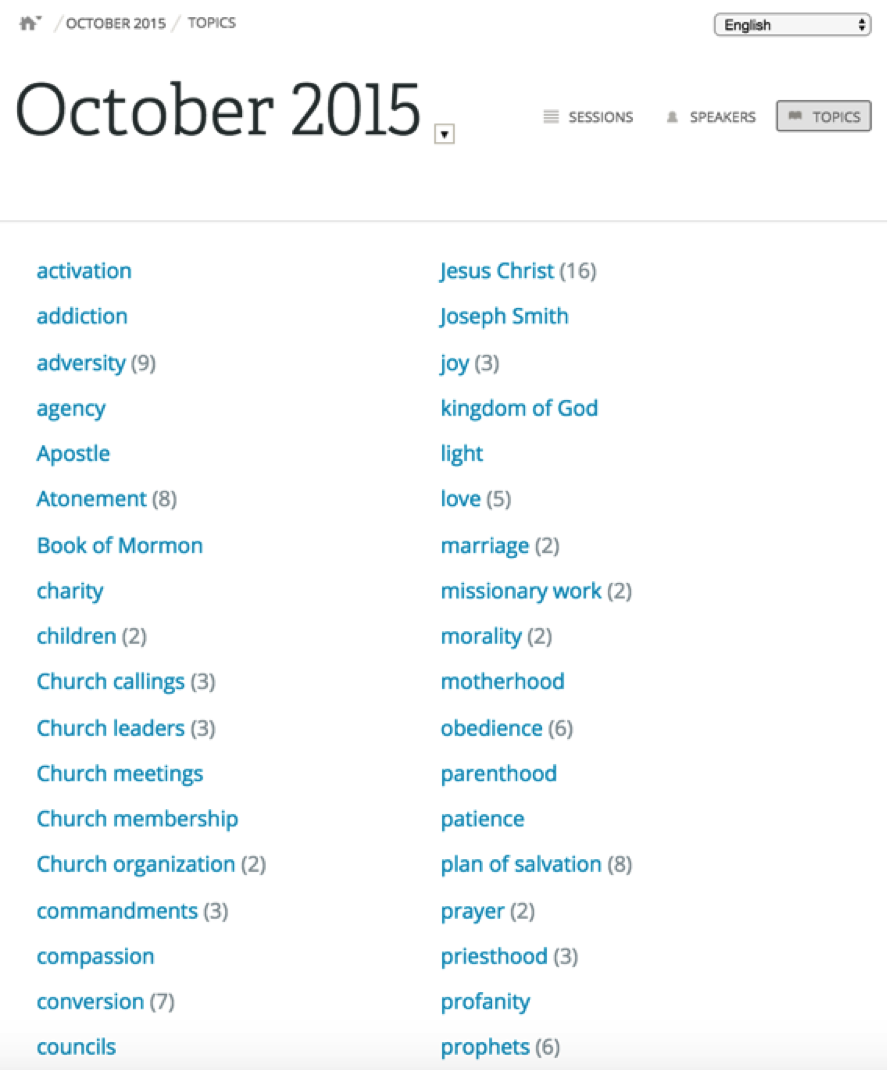
\includegraphics[width=4.5in,natwidth=410,natheight=542]{figures/oct_2015_topics.png}
		\caption[\url{LDS.org} 2015 Topics]{
			\url{LDS.org} 2015 Topics
		}
	\label{fig:oct_2015_topics}
\end{figure}

Therefore, for users of \url{LDS.org}, when a reader enjoys a particular discourse, it is difficult to locate all discourses on a given topic. It is theoretically possible to peruse every session of GC (as far back as 1971) looking for the topic for every year. The task requires a lot of clicking and will not work for discourses published before 1971 since they are not exposed online at \url{LDS.org}.

Beyond the per-year topic index provided by \url{LDS.org}, \url{LDS.org} does have a Gospel Topics index at \url{https://www.lds.org/topics/}. Under some topics, there are discourses that are selected for the topic, but they don’t promise to be results of a recommendation system--and expanding the lists to see more is not possible.

\emph{LDS SCI} has discourses by topic, but was manually created and only accounts for discourses in the Journal of Discourses, which were published in the 1800’s. For those interested, digital images of the Journal of Discourses is available from the BYU online collections at \url{http://contentdm.lib.byu.edu/cdm/search/collection/JournalOfDiscourses3}.

To review, \url{LDS.org} has 2 topic indexes, one of which focuses on a per-year approach for post-1971 GC talks, the other of which appears to have been manually created. \emph{LDS SCI} has a topic index, but only for very early discourses. For a superficial study of a topic, this might be sufficient, but when one wants to reach farther than the most recent or least LDS materials--namely those in the middle--there is no search engine--and none which promises to be automatic, automatically updated, and interactive.

In the past 2 years, the query engine provided by both \url{LDS.org} and \emph{LDS SCI} have been enhanced significantly, but they still leave something to be desired: simplicity and ease of use. Dr. Liddle who built \emph{LDS SCI} has said that \emph{LDS SCI} uses a Lucene query engine, which employs a \emph{TF-IDF} search algorithm. The \url{LDS.org} engine seems to work similarly, except that it can detect phrases such as ``in talks'' and use those to automatically select to search only through discourses rather than through all LDS written materials exposed online. [...more on how LDS SCI search engine works...]

Take for example the search query ``word of wisdom'' (without quotes in the search). This is a phrase which is more recent history of the LDS church has come to refer to a law of health. The search results look promising:

\begin{figure}[hhhhhtb]
	\centering
		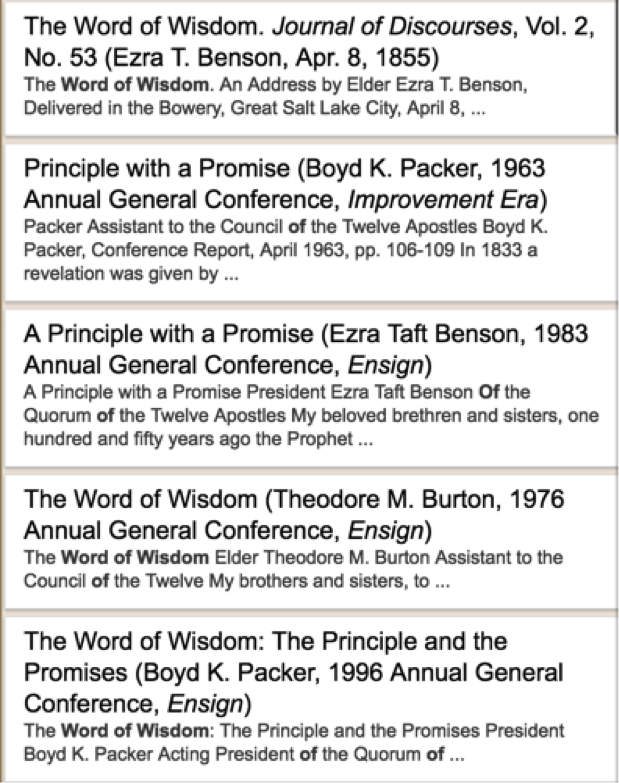
\includegraphics[width=3.5in,natwidth=310,natheight=442]{figures/sci_results.png}
		\caption[Top SCI Query Results for the search \textit{Word of Wisdom}]{

		}
	\label{fig:sci_results}
\end{figure}

But one would expect to see something by Joseph Smith Jr. to rank at the top. The confounding factor here is that ``word of wisdom'' is a modern naming convention. % TODO: Fact check this!
The word of wisdom was ``[r]evelation given through Joseph Smith the Prophet, at Kirtland, Ohio, February 27, 1833.'' (D\&C 89 Header). The earliest usage of the phrase ``word of wisdom'' in print we could find is 1873--40 years after it was revealed. (TODO: cite The Word of Wisdom—Education by President George A. Smith).

Unfortunately, without a way to determine what topics exist within all the LDS discourses, there is no way for a query system to expand queries like this one. Unfortunately, even if the user does happen to find a discourse that is a pleasing match to the query, there is currently no recommendation system from that point to suggest other related discourses--just existing links and the other results for the query.

If the user were to filter to only scriptures, they would find more than 20k matches:

\begin{figure}[hhhhhtb]
	\centering
		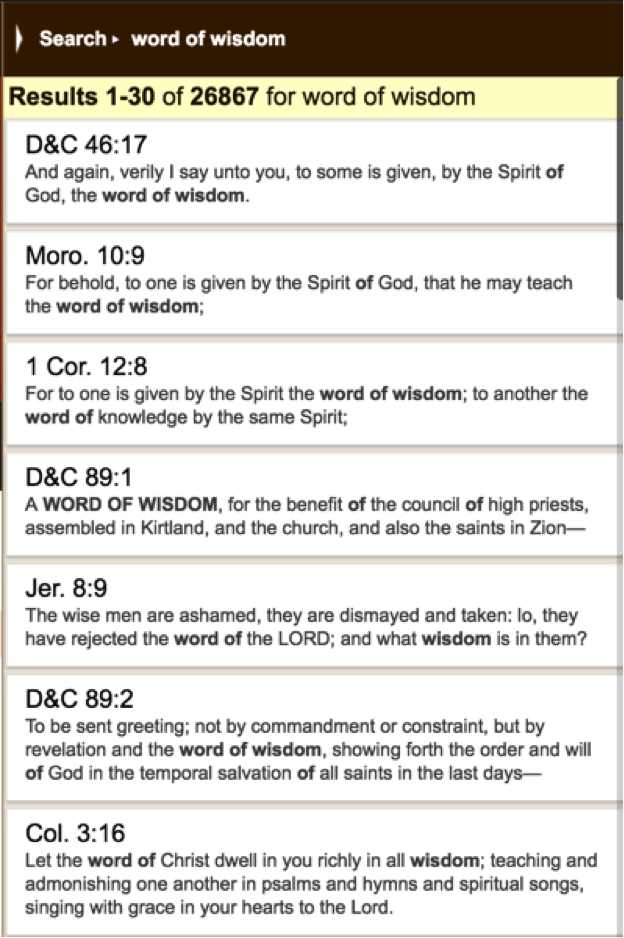
\includegraphics[width=3.5in,natwidth=310,natheight=442]{figures/sci_results_20k.png}
		\caption[20k+ SCI Results]{

		}
	\label{fig:sci_results_20k}
\end{figure}

Of those, the first one that refers to directly to a law of health is the 4th result. \url{LDS.org}, when performing the same search ranks the result referring to the law of health as the 4th result (\url{https://www.lds.org/scriptures/search?type=verse&query=word+of+wisdom}), but does so with only 39 total results. These are results that I was able to find because I understood how the search engine works. When one doesn’t know when to put quotes or doesn’t know what they are looking for, the task is more difficult, depending on the engine used. For example, when the entire query is run with quotes around it in \emph{LDS SCI}, the number of results drops from the 20k down to 7 in \emph{LDS SCI} and in \url{LDS.org} down from 39 to 8 in \url{LDS.org} (\url{https://www.lds.org/scriptures/search?type=verse&query="word+of+wisdom"}). [Search relevance is an entire area of research and it is no wonder that companies that are able to do well in this area are able to profit from it (e.g. Microsoft with \url{https://bing.com} and Google with \url{https://google.com}).]

While search query optimization would be one way to improve this area, I chose to augment the \emph{LDS SCI} toolset with recommendation features. The idea was that once a reader locates a discourse of interest, it would be helpful to provide a list of similar discourses as a list. The list could default to displaying 5, but the user could interact with the result and request additional results. There are many ways to approach this that I will explain.

Attempting to do the same for all portions of the process, \citeauthor{bean5-plagiarism-detection} used a combined approach of gene sequence alignments and machine learning to automatically identify alignment positions of intertext. Topic modeling was not used which might explain why the system performed poorly. Word sense disambiguation was not used either, but WordNet synsets were used \citep{wordnet_1998}. The corpus was religious in nature. Some of the documents had been translated manually, which probably introduced a significant amount of noise. Like the work of Hilton III, Bean’s work could probably have benefited from the use of LDA or word sense disambiguation.

\section{Recommender Systems}

In this section I give a sampling of topics to be more fully explored in the full thesis document.
One way to produce recommendations for textual data is by using post-hoc methods built on topic modeling \citep{blei2012probabilistic}. One well-known topic model is Latent Dirichlet Allocation, or \emph{LDA}, which is a model of word-topic assignments. From this model post-hoc algorithms extract various meta-data including probability of a topic (overall or in a document), and probability of a word in a topic. This step is fast and effective. Given a probability distribution over topics, machine learning approaches including nearest neighbor approaches (e.g. k-NN) can locate the most relevant documents. Since probability distributions are points that exist within the \textit{Probability Simplex}, or \emph{T}-space \citep{Krstovski2013efficient} metrics suited for the space such as the \emph{Jensen-Shannon divergence} or the \emph{Hellinger distance} are viable metrics for determining distance between points. Distance is interpreted as dissimilarity (i.e. closer points are considered more similar than two distant points).

Topic models are not required for document recommendation. Algorithms that use token frequency and inverse document frequency, or \emph{TF-IDF}, can also be used. In such cases, documents with the similar distributions of keywords can be considered similar.

A subset of topic modeling aims to analyze topical trends over time. Such work includes that of \citep{hall-jurafsky-manning:2008:EMNLP} where entropy, applied on chronological disjoint sets of texts, is used as a metric of showing broadening/narrowing of topics over time. They demonstrated that the \emph{Jensen-Shannon divergence} divergence between venue \emph{venue pairings}\footnote{or disjoint sets of documents} could be used to measure level of similarity. They aptly demonstrated that topic entropy, when applied to topics on a per-year basis, could be used to describe the ebb and flow of each topic’s \emph{popularity} over time. As a result, entropy of entire scholarly conferences can be plotted over time and compared. They showed that two separate conferences were converging to the have similar entropy of topics as time progressed.

In precursory work, by following the methods outlined by \cite{hall-jurafsky-manning:2008:EMNLP}, I found that the same technique could be generalized further. Instead of dividing data into venues based on conference, I divided based on gender of author, then further divided based on year of authorship. Like this work, LDA was run on this same dataset. After some trial and error, I determined that 150 was appropriate for the number of expected topics \citep{bean5-LDA-ToT}.%(Bean and Ringger, 2013).

\cite{Krstovski2013efficient} %Krstovski (2013)
shows that it is possible to efficiently apply speed-up k-NN algorithms to the other- wise slow process of obtaining the closest \emph{k} neighbors. Although they primarily tested their hypothesis using contrived datasets, it is convincing enough for us to use the same distance metric in this work. In the probability simplex where probability distributions are over topics, this the distance metric shows how similar two documents are in terms of topic content. When running k-NN, whenever two documents are close to each other in the space, they are considered related.

Less automated text mining on LDS religious documents includes \citep{hilton:2008:abinadi} %Hilton III (2008)
. \citeauthor{hilton:2008:abinadi} aimed to discover what he calls intertextual similarity between authors of LDS-specific texts. In his work, he focused on \emph{The Book of Mormon}, although he later demonstrated that the methodology could locate results between \emph{The Holy Bible} and \emph{The Book of Mormon} \citep{hilton:2013:psalms}. Although topic models were not employed in his work, it probably could have benefited from them. Computational methods were involved, but only for portions of the process.

% TODO: Before referencing LDA, describe it or use longer name.
Recommender systems, sometimes called recommendation systems, vary in the way that they are created. For this work, two possible systems stood out immediately for my use: LDA-based recommendation and \emph{TF-IDF} based recommendation. The latter is straightforward, easy to implement, and uses the same metrics that the query search at \emph{LDS SCI} uses. The LDA-based model brings additional features to the table, but does so indirectly. Every LDA is a distribution over distributions. In my case, for the model to be built, each word token is assigned to a 1 and only 1 topic. This can easily be collected and indexed, then exposed as a keyword frequency index for each topic. So on top of providing per-discourse recommendations, it could easily be used to create an index of topics, linkable to the documents with a large clustering of words in each topic! Since that was not a main focus in my work, I published the results of that at \url{http://bean5.github.io/lds-talks-by-topic/} for future use. The downside to LDA is that it is only a model. An algorithm to building the LDA model must be selected. Some algorithms include:

\begin{enumerate}
  \item Gibbs Sampling, a Markov chain Monte Carlo algorithm
  \item Variational Inference; and
  \item Expectation Maximization
\end{enumerate}

The LDA and \emph{TF-IDF} model share some similarities besides lending themselves as models for recommender algorithms. They treat each document as a bag of words. They can both be told to ignore common words, although the nature of \emph{TF-IDF} is such that high frequency words are not as noisy or problematic as they are for LDA models.

...

Running a Gibbs Sampler long enough is guaranteed to converge to what is called the posterior. A good initialization makes it converge sooner, but in previous work, we found that 1000 iterations of Gibbs converged well to a good set of topics (see elsewhere; \url{https://youtu.be/UTW530-QVxo?t=1189}).

\section{Algorithms}
\begin{enumerate}
  \item k-NN
  \item ...
\end{enumerate}

\section{Metrics}
\begin{enumerate}
  \item k-NN metrics
  \item Jenson-Shannon
  \item Hellinger distance (Jenson-Shannon reduced for parallelization in k-NN; produces same results as Jenson-Shannon when used in k-NN)
\end{enumerate}

\section{LDA}
LDA stands for latent dirichlet allocation. It is a model where each token within a document is tagged with 1 and only 1 topic. Each document is treated as a bag of words.

\section{Evaluation}

Many metrics exist for the purpose of measuring \textit{goodness} of results. When ordered sets constitute the output, which is the case for search and discovery-based methods, \textit{precision} and \textit{recall} are two commonly trusted metrics. A way to balance them is to compute the F1 \textit{score} or \textit{f-measure}, which is simply the harmonic mean of the two. It is important to note that these metrics only work when a gold standard exists, e.g. when the best results are known a-priori for some test portion of the dataset. Metrics which do not require a gold standard include \textit{catalog coverage}. The \textit{serendipity} metric requires at least a baseline set of recommendations (Ge et al., 2010).

Catalog coverage metrics show how good a system is at providing results throughout the system rather than favoring certain documents. \textit{Serendipity} measures how good a system is at producing results that are surprising rather than obvious. I will use the formulas as provided by and described by Ge et al. (2010).

When \textit{comparing} the output sets of two systems, a gold standard does not have to exist. If the two perform similarly, they will have similar output. One can measure similarity using formulas in the nDCG family (Wang et al., 2013). This can lend credibility to either system if one tends to provide output that is similar to the already-accepted system.

\section{Problems}
\[TODO: Complete this section.\]

\section{Open Source Tools: Docker, Mallet, npm}
Core to this project is the use of docker. Dockers are Linux containers which the docker-engine (i.e. docker daemon) can build and run. They can be thought of as Linux virtual machines in some ways, although they tend to be resource/hardware agnostic since they simply share the kernel, RAM, and other hardware on the host on which they are run. They are considered lightweight since instead of running the full Linux stack for each container, only necessary files are run from within the container. This has made it easy for a new market to emerge where products that are software as a service (SaaS) can be hosted at a lower cost. Container Engine by Google (\url{https://cloud.google.com/container-engine/}) and tutum but Tutum (\url{https://www.tutum.co/}) are examples of this.

% TODO: Cite quote instead of linking
Docker has a growing community around it. In fact, Google has created an open source project called Kubernetes which aims to ``accelerate Dev and simplify Ops'' (\url{https://kubernetes.io/}). It is used under the covers for Container Engine, a Google cloud product. Although Linux containers have been around for some time now, the docker community has made it much more mainstream, especially for computing environments where scaling horizontally is important. Thus, companies such as Netflix, EMC find it highly beneficial. In my experience, Linux tools with growing communities are well backed, become robust, and tend to be both easy to use as well as empowering.
Docker has quickly become that. Use in this thesis is one evidenced of its growing popularity. % TODO: Move to methodology section.
